\documentclass[a4paper, 12pt]{article}
\usepackage{graphicx}
\usepackage[utf8]{inputenc}
\usepackage[ukrainian]{babel}
\usepackage{amsmath}
\usepackage{fancyhdr}
\usepackage{geometry}
\geometry{top=2cm, bottom=2cm, left=3cm, right=1.5cm}
\usepackage[colorlinks=true,linkcolor=blue]{hyperref}%
\usepackage{caption}
\DeclareCaptionType[within=section]{mat}[]
\begin{document}

\begin{titlepage}
	\begin{center}
		\Large
		\textbf{Київський національний університет імені Тараса Шевченка} \\
		Факультет комп'ютерних наук та кібернетики \\

		\vspace{6cm}

		\textbf{\LARGE ЗВІТ ДО ЛАБОРАТОРНОЇ РОБОТИ №3} \\[0.5cm]
		\textbf{З дисципліни ``Чисельні методи''} \\[0.5cm]
		\textbf{Тема: Розв'язування системи нелінійних алгебраїчних рівнянь} \\

		\vfill
		\hspace{7cm} Виконав студент 3-го курсу \\
		\hspace{7cm} групи ТТП-31 \\
		\hspace{7cm} Рісенгін Владислав \\
		\vspace{2cm}

		Київ-2024
	\end{center}
\end{titlepage}

\newpage

\hbadness=99999

\section{Постановка задачі}

Придумати систему яка складається з 3 нелінійних рівнянь. І вектором правої частини $\overline f = (0, 0, 0)$. \\

Розв'язати її методом простої ітерації, і модифікованим методом Ньютона

\section{Вступ}

Метою цієї лабораторної роботи є вивчення методів розв'язування системи нелінійних алгебраїчних рівнянь, 
які дають можливість вирішення багатьох наукових та інженерних задач. \\

У процесі виконання роботи будуть досліджені та реалізовані методи простої ітерації, модифікований метод Нютона.

\section{Деталі реалізації}

Лабораторна робота виконана використовуючи мову програмування Python, а також бібліотеку numpy.

\clearpage
\section{Теоретичний опис методів}
% \subsection{Метод простої ітерації}

\begin{figure}[ht]
	\centering
	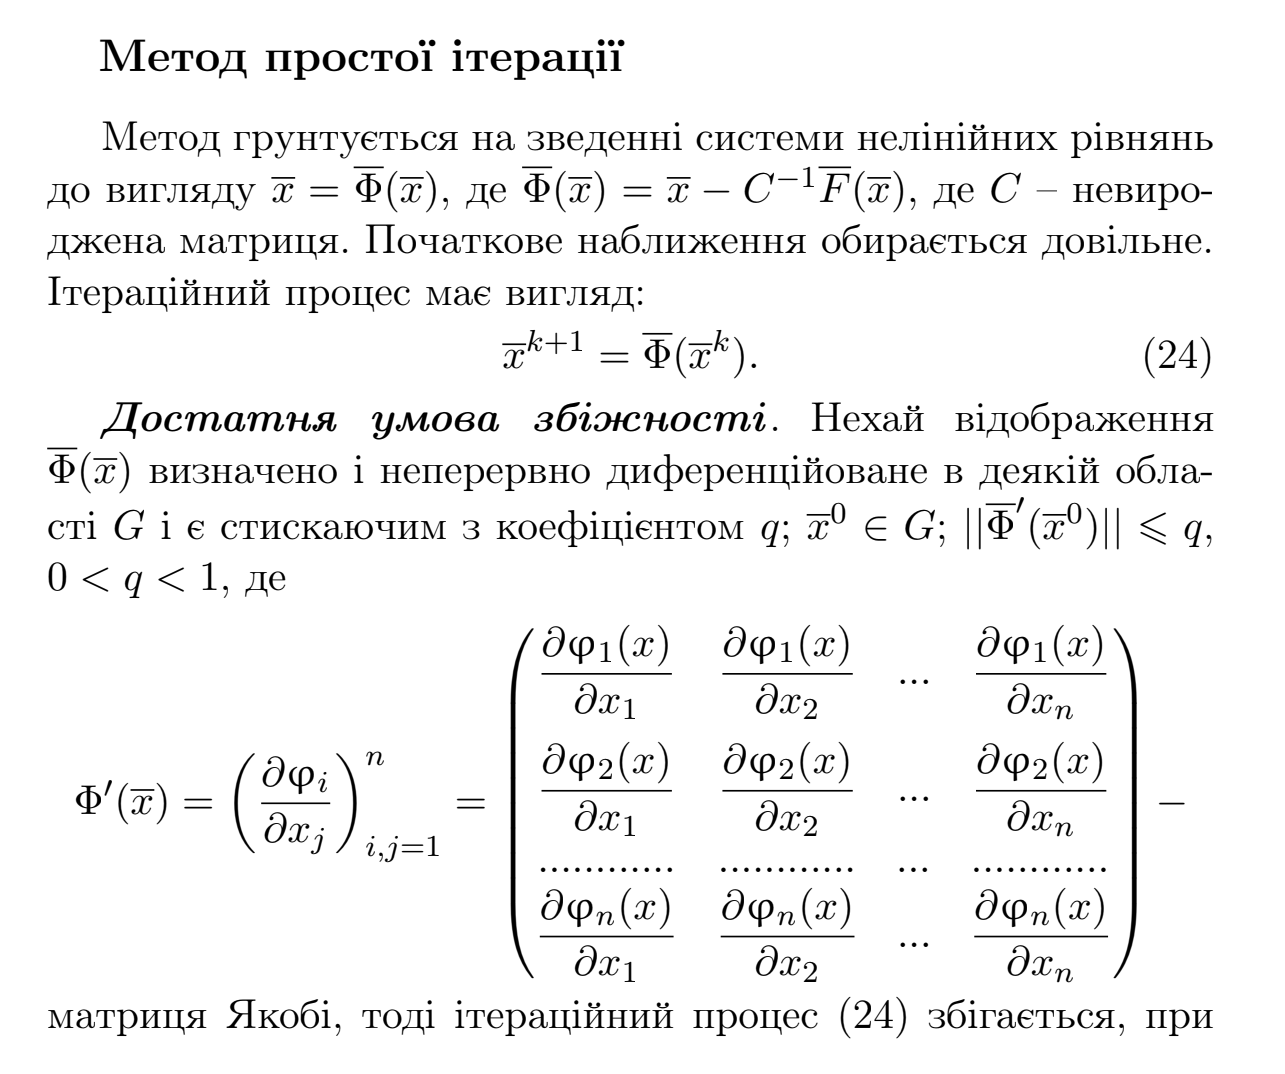
\includegraphics[width=0.9\linewidth]{iteration1.png}
\end{figure}
\begin{figure}[ht]
	\centering
	
\includegraphics[width=0.9\linewidth]{iteration2.png}
\end{figure}

\clearpage
\newpage
% \subsection{Модифікований метод Ньютона}

\begin{figure}[ht]
	\centering
	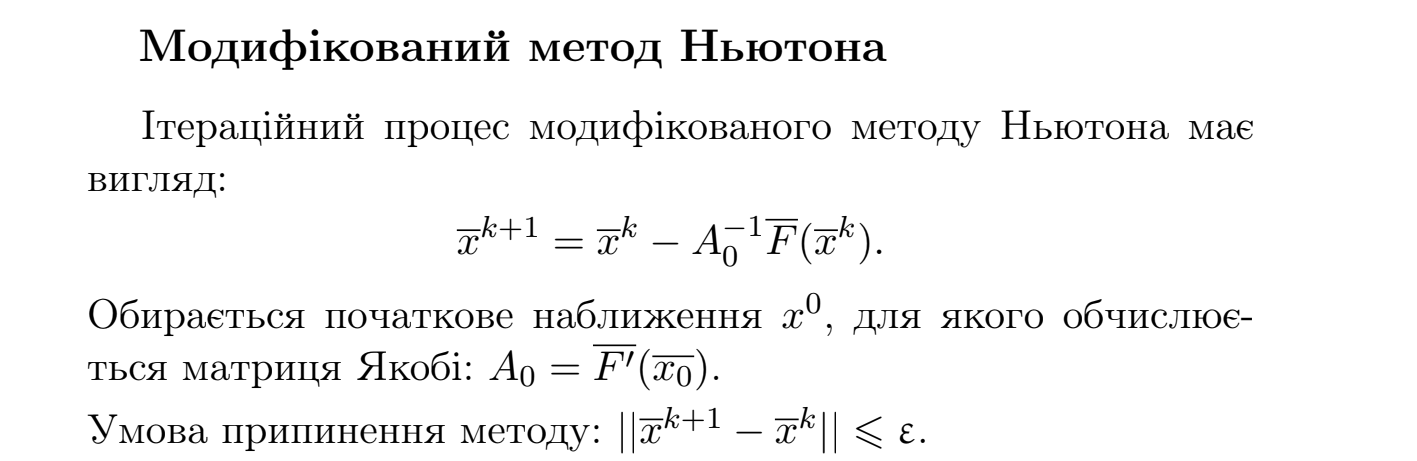
\includegraphics[width=0.9\linewidth]{mod_nuton1.png}
\end{figure}

\newpage

\section{Результати роботи програми}

Для методу простої ітерації будемо шукати розв'язок з точністю $\epsilon = 10^{-4}$ \\
Для модифікованого методу Ньютона будемо шукати розв'язок з точністю $\epsilon = 10^{-6}$ \\

Як критерій зупинки використовується $||\overline x^{k+1} - \overline x^k || < \epsilon $ 
\begin{center}
    \( \|\overline{x}\| = \max(|x_1|, |x_2|, \dots, |x_n|) \)
\end{center}

Система F для розв'язання: 

\begin{equation}
	\begin{cases}
	3x_1 - \sin(x_2) - \frac{1}{e^{x_3}} = 0, \\
	5x_2 + \cos(x_1) - x_3^2 = 0, \\
	4x_3 + x_1^2 - x_2 = 0.
	\end{cases}
	\label{eq:F}
\end{equation}


\subsection{Метод простої ітерації}

Оберемо початкове наближення \(\overline x_0 = [0.5, -0.5, -0.5]\)

\[ \overline x^{k+1} = \overline{x}^k - C(\overline x^k) \overline F(\overline x^k) \]

\begin{equation}
	\begin{bmatrix}
		0.1 + x_1/1000 & 0 & 0  \\ 
		0 & 0.1 + x_2/1000 & 0  \\ 
		0 & 0 & 0.1 + x_3/1000  \\ 
	\end{bmatrix}
\end{equation}
\captionof{mat}{Матриця C}

\begin{verbatim}
Iteration  |                  x_new                   |    Norm   
----------------------------------------------------------------------
0          | [ 0.500000 -0.500000 -0.500000]          | -
1          | [ 0.466764 -0.313694 -0.375625]          | 0.186305535
2          | [ 0.441349 -0.232297 -0.278896]          | 0.096728962
3          | [ 0.417988 -0.198866 -0.210238]          | 0.068657772
4          | [ 0.396142 -0.186428 -0.163599]          | 0.046639121
5          | [ 0.376461 -0.182800 -0.132546]          | 0.031053100
6          | [ 0.359454 -0.182641 -0.112007]          | 0.020538869
7          | [ 0.345256 -0.183673 -0.098404]          | 0.014197534
8          | [ 0.333716 -0.184965 -0.089339]          | 0.011539822
9          | [ 0.324525 -0.186165 -0.083242]          | 0.009191488
10         | [ 0.317315 -0.187168 -0.079097]          | 0.007209433
11         | [ 0.311726 -0.187965 -0.076246]          | 0.005589078
12         | [ 0.307432 -0.188580 -0.074263]          | 0.004294377
13         | [ 0.304155 -0.189049 -0.072868]          | 0.003277065
14         | [ 0.301667 -0.189403 -0.071878]          | 0.002487609
15         | [ 0.299786 -0.189669 -0.071168]          | 0.001880689
16         | [ 0.298369 -0.189867 -0.070655]          | 0.001417404
17         | [ 0.297303 -0.190016 -0.070282]          | 0.001065672
18         | [ 0.296504 -0.190127 -0.070010]          | 0.000799736
19         | [ 0.295904 -0.190209 -0.069810]          | 0.000599307
20         | [ 0.295456 -0.190271 -0.069663]          | 0.000448615
21         | [ 0.295120 -0.190317 -0.069555]          | 0.000335530
22         | [ 0.294869 -0.190351 -0.069474]          | 0.000250789
23         | [ 0.294682 -0.190377 -0.069414]          | 0.000187356
24         | [ 0.294542 -0.190396 -0.069370]          | 0.000139915
25         | [ 0.294438 -0.190410 -0.069337]          | 0.000104456
26         | [ 0.294360 -0.190421 -0.069313]          | 0.000077966
\end{verbatim}

Збіжність досягнута після 26 ітерацій. \\
Розв'язок: 
\( \overline x = ( 0.2943597515255351, -0.1904209166651033, -0.0693127420138911 )^T \)

Перевірка результату: \\
\(\overline F(\overline{x}) = ( 5.8013008962065626e-04, 7.9252417547879227e-05, -1.8238807228646015e-04)^T \)

\newpage
\subsection{Модифікований метод Ньютона}

Оберемо початкове наближення \(\overline x_0 = [0.5, -0.5, -0.5]\) \\

Обчислимо Якобіант 

\begin{equation}
	\begin{bmatrix}
		3 & -cos(x_2) & e^{x_3} \\
		-sin(x_1) & 5 & -2 x_3 \\
		2 x_1 & -1 & 4 \\
	\end{bmatrix}
\end{equation}
\captionof{mat}{Матриця \(A_k\)}

Підставимо \(x_0\) в \(A_0\)

\begin{equation}
	\begin{bmatrix}
		3 & -0.8775825618903728 & 0.6065306597126334 \\ 
		-0.479425538604203 & 5 & 1 \\
		1 & -1 & 4  \\
	\end{bmatrix}
\end{equation}
\captionof{mat}{Матриця \(A_0\)}

Знайдемо обернену матрицю 

 \begin{equation}
	\begin{bmatrix}
		0.3639665587739987 &  0.0503279020647002 & -0.0677711947678076 \\
		0.0505688577462176 &  0.1974686584895931 & -0.0570350552848302 \\
		-0.0783494252569453 & 0.0367851891062232 &  0.2526840348707444 \\
	\end{bmatrix}
\end{equation}
\captionof{mat}{Матриця \(A^{-1}_0\)}


\[ \overline x^{k+1} = \overline{x}^k - A^{-1}_0 \overline F(\overline x^k) \]


\begin{verbatim}
Iteration  |                  x_new                   |    Norm   
----------------------------------------------------------------------
0          | [ 0.500000 -0.500000 -0.500000]          | -
1          | [ 0.389156 -0.218273 -0.089357]          | 0.410642762
2          | [ 0.293005 -0.197881 -0.063293]          | 0.096150894
3          | [ 0.293152 -0.189542 -0.068885]          | 0.008339017
4          | [ 0.294157 -0.190335 -0.069320]          | 0.001004910
5          | [ 0.294144 -0.190465 -0.069245]          | 0.000129223
6          | [ 0.294130 -0.190453 -0.069240]          | 0.000013820
7          | [ 0.294130 -0.190452 -0.069241]          | 0.000001613
8          | [ 0.294131 -0.190452 -0.069241]          | 0.000000188
\end{verbatim}

Збіжність досягнута після 8 ітерацій. \\
Розв'язок: 
\( \overline x = ( 0.2941306455006774, -0.1904520207886972, -0.0692412336722941)^T \)

Перевірка результату: \\
\(\overline F(\overline{x}) = (-8.319434918746538e-09, 8.433744491404688e-08, -7.727783385425013e-08)^T \)

\newpage
\section{Висновок}

У результаті роботи обох методів було досягнуто розв'язку з необхідною точністю. \\ 

Метод простої ітерації виявився менш ефективним, потребуючи 26 ітерацій для досягнення збіжності. \\ 
Розв'язок: \( \overline x = ( 0.2943597515255351, -0.1904209166651033, -0.0693127420138911 )^T \)
 пройшов перевірку, показавши значення функцій, близькі до нуля, що свідчить про правильність розв'язку. \\ 

З іншого боку, модифікований метод Ньютона виявився значно швидшим, досягнувши збіжності вже за 8 ітерацій. \\ 
Розв'язок: \( \overline x = ( 0.2941306455006774, -0.1904520207886972, -0.0692412336722941)^T \) \\
 також продемонстрував значення функцій близькі до 0, підтверджуючи його коректність. \\ 

Отже, можна стверджувати, що модифікований метод Ньютона є більш ефективним у даному випадку, забезпечуючи швидшу збіжність і високу точність розв'язку в порівнянні з методом простої ітерації. \\ 

Це підкреслює важливість вибору відповідних чисельних методів для розв'язання нелінійних систем рівнянь, залежно від їхніх властивостей та вимог до точності.

\end{document}
